\documentclass[11pt]{article}
\usepackage{mathblatt}
% gesetzt von werkzeuge/setzer.py (Sorte selbst) aus dem Lernweg FP6
% und den Bankzeilen; Muster bau/proben/2026-10-09/hypotenuse-muster.
\usepackage{enumitem}
\usepackage{adjustbox,varwidth}
\newgeometry{a4paper,margin=18mm,top=15mm,bottom=20mm,footskip=9mm}
\pagestyle{fancy}\fancyhf{}\renewcommand{\headrulewidth}{0pt}
\fancyfoot[L]{\footnotesize\color{mbgrau}FP6 \textperiodcentered{} Winkel an Geradenkreuzungen und Parallelen}
\fancyfoot[R]{\footnotesize\color{mbgrau}\thepage}
\setlength{\parskip}{3pt}
\renewcommand{\kreuz}[1]{\mbox{$\square$\ #1}\quad}
\newcommand{\kreuzl}[1]{\par\hangindent1.4em\hangafter1\noindent$\square$\ #1}
\newcommand{\aufg}[3]{\par\noindent\makebox[0pt][r]{#3}\begin{minipage}[t]{\linewidth}#1\end{minipage}\par}
\newcommand{\aufgg}[4]{\par\noindent\makebox[0pt][r]{#4}\begin{minipage}[t]{0.6\linewidth}\vspace{0pt}#1\end{minipage}\hfill
  \begin{minipage}[t]{0.37\linewidth}\vspace{0pt}\centering #2\end{minipage}\par}
\newcommand{\nr}[1]{\makebox[7mm][l]{\textbf{#1}}}
\newcommand{\lsg}[3]{\par\noindent\begin{minipage}[t]{9mm}\textbf{#1}\end{minipage}%
  \begin{minipage}[t]{52mm}\raggedright\bfseries\boldmath #2\end{minipage}\hspace{3mm}%
  \begin{minipage}[t]{\dimexpr\linewidth-64mm\relax}\raggedright\small #3\end{minipage}\par\vspace{4pt}}
\newlength{\kr}
\makeatletter
\newcommand{\karomerk}[2]{\protected@write\@auxout{}{\string\karoseite{#1}{#2}{\thepage}}}
\newcommand{\karoseite}[3]{\expandafter\xdef\csname karo@#1@#2\endcsname{#3}}
\newcommand{\karohinweis}[3]{\karomerk{h}{#1}\ifcsname karo@k@#1\endcsname
  \ifnum\csname karo@k@#1\endcsname=0\csname karo@h@#1\endcsname\relax#2\else#3\fi
  \else#3\fi}
\makeatother
\begin{document}

\noindent{\LARGE\bfseries Winkel an Geradenkreuzungen und Parallelen}\par\smallskip
\noindent{\small\color{mbgrau}Selbstlernheft Klasse 7 \textperiodcentered{} mit Lösungsheft \textperiodcentered{} Kennung FP6}\par\medskip
\noindent\textbf{So nutzt du das Heft:} Lies im Abschnitt das Beispiel. Rechne dann die Aufgaben der Reihe nach und vergleiche jede sofort mit dem Lösungsheft. Kreuze „kann ich“ an, wenn du die letzte Aufgabe (\emph{Ziel}) allein schaffst.\par
\noindent Mehr Aufgaben zu einem Abschnitt: Kennung deinem Nachhilfelehrer schicken (z.\,B. „FP6 mehr B“).\par\medskip
{\arrayrulecolor{mbgrau}\renewcommand{\arraystretch}{1.3}
\noindent\begin{tabular}{|>{\bfseries}p{10mm}|p{112mm}|>{\raggedleft\arraybackslash}p{10mm}|>{\centering\arraybackslash}p{14mm}|}\hline
\rowcolor{black!8} & \textbf{Abschnitt} & \textbf{Seite} & \textbf{kann ich}\\\hline
A & Scheitel- und Nebenwinkel & \pageref{s:A} & $\square$\\\hline
B & Kreuzungen in Figuren & \pageref{s:B} & $\square$\\\hline
C & Winkel an Parallelen & \pageref{s:C} & $\square$\\\hline
D & Parallelogramm und Trapez & \pageref{s:D} & $\square$\\\hline
T & Probetest & \pageref{s:T} & $\square$\\\hline
\end{tabular}}\par\bigskip

\begin{tcolorbox}[colback=mbkasten,colframe=mbgrau,boxrule=0.5pt,arc=1mm,left=3mm,right=3mm,top=2mm,bottom=2mm,title={\bfseries Formel auf einen Blick},coltitle=black,colbacktitle=black!10]
\begin{minipage}[t]{0.58\linewidth}\vspace{0pt}
{\Large gegenüber: gleich groß\par daneben: zusammen $180^\circ$}\par\medskip
In Worten: Fast jede Aufgabe läuft auf eine Frage hinaus: Ist der gesuchte Winkel so groß wie ein bekannter – oder ergänzt er ihn zu $180^\circ$?\par\medskip
\textbf{So gehst du vor}\par
\nr{1}die zwei Geraden suchen, an denen der gesuchte Winkel liegt\par
\nr{2}einen bekannten Winkel an derselben Kreuzung suchen\par
\nr{3}Lage benennen: gegenüber oder daneben\par
\nr{4}rechnen, Gradzeichen dazu\par
\medskip
\end{minipage}\hfill
\begin{minipage}[t]{0.38\linewidth}\vspace{2mm}\centering
\begin{tikzpicture}[line width=0.7pt,font=\small]\draw (0,0) -- (1.04,0);\draw (0,0) -- (0.44,0.943);\draw (0,0) -- (-1.04,0);\draw (0,0) -- (-0.44,-0.943);\draw[mbgrau,line width=0.5pt] (0.42,0) arc (0:65:0.42);\node[inner sep=0pt] at (0.582,0.371) {$\alpha$};\draw[mbgrau,line width=0.5pt] (0.177,0.381) arc (65:180:0.42);\node[inner sep=0pt] at (-0.371,0.582) {$\beta$};\draw[mbgrau,line width=0.5pt] (-0.42,0) arc (180:245:0.42);\node[inner sep=0pt] at (-0.582,-0.371) {$\gamma$};\draw[mbgrau,line width=0.5pt] (-0.177,-0.381) arc (245:360:0.42);\node[inner sep=0pt] at (0.371,-0.582) {$\delta$};\fill (0,0) circle (1.3pt);\end{tikzpicture}
\end{minipage}
\end{tcolorbox}
\medskip\noindent\textbf{Typische Fehler – so nicht}\par\smallskip
\noindent\nr{$\times$}Nebenwinkel statt Scheitelwinkel: $180^\circ - 74^\circ$ gerechnet, obwohl der Winkel gegenüberliegt. Gegenüber heißt gleich groß.\par
\noindent\nr{$\times$}Stufenwinkel abgeschrieben, obwohl der Winkel daneben gefragt ist: $53^\circ$ statt $127^\circ$. Schau nach, wo der gesuchte Winkel liegt.\par
\noindent\nr{$\times$}Teilwinkel: $180^\circ - 50^\circ - 30^\circ$ statt $50^\circ - 30^\circ$. Erst den ganzen Winkel, dann den Teil abziehen.\par
\clearpage\label{s:A}\noindent\colorbox{black!12}{\makebox[10mm]{\Large\bfseries\strut A}}\hspace{3mm}{\Large\bfseries Scheitel- und Nebenwinkel}\par\smallskip
\noindent Kreuzen sich zwei Geraden, entstehen vier Winkel. Gegenüberliegende Winkel heißen \textbf{Scheitelwinkel}, nebeneinanderliegende \textbf{Nebenwinkel}.\par\medskip
\noindent\textbf{Formel}\par\nopagebreak\noindent\hspace*{4mm}\begin{minipage}{\dimexpr\linewidth-4mm\relax}Scheitelwinkel sind gleich groß: \ $\gamma = \alpha$ \qquad Nebenwinkel ergeben zusammen $180^\circ$: \ $\beta = 180^\circ - \alpha$\end{minipage}\par\medskip
\noindent\textbf{Beispiel}\quad Zwei Geraden kreuzen sich. Es ist $\alpha = 65^\circ$. Berechne $\beta$, $\gamma$ und $\delta$.\par\smallskip
\noindent\begin{minipage}[t]{0.6\linewidth}\vspace{0pt}\par\noindent\hangindent6mm\hangafter1\makebox[6mm][l]{\textbf{1}}$\gamma$ liegt $\alpha$ gegenüber: \textbf{Scheitelwinkel}. \ $\gamma = 65^\circ$\par\smallskip\par\noindent\hangindent6mm\hangafter1\makebox[6mm][l]{\textbf{2}}$\beta$ liegt neben $\alpha$: \textbf{Nebenwinkel}. \ $\beta = 180^\circ - 65^\circ = 115^\circ$\par\smallskip\par\noindent\hangindent6mm\hangafter1\makebox[6mm][l]{\textbf{3}}$\delta$ liegt $\beta$ gegenüber: \ $\delta = 115^\circ$\par\smallskip\end{minipage}\hfill
\begin{minipage}[t]{0.37\linewidth}\vspace{0pt}\centering \begin{tikzpicture}[line width=0.7pt,font=\small]\draw (0,0) -- (1.04,0);\draw (0,0) -- (0.44,0.943);\draw (0,0) -- (-1.04,0);\draw (0,0) -- (-0.44,-0.943);\draw[mbgrau,line width=0.5pt] (0.42,0) arc (0:65:0.42);\node[inner sep=0pt] at (0.582,0.371) {$\alpha$};\draw[mbgrau,line width=0.5pt] (0.177,0.381) arc (65:180:0.42);\node[inner sep=0pt] at (-0.371,0.582) {$\beta$};\draw[mbgrau,line width=0.5pt] (-0.42,0) arc (180:245:0.42);\node[inner sep=0pt] at (-0.582,-0.371) {$\gamma$};\draw[mbgrau,line width=0.5pt] (-0.177,-0.381) arc (245:360:0.42);\node[inner sep=0pt] at (0.371,-0.582) {$\delta$};\fill (0,0) circle (1.3pt);\end{tikzpicture}\end{minipage}\par\medskip
\noindent\textbf{Aufgaben}\hspace{1em}{\small\color{mbgrau}\karohinweis{A}{Rechne unten im Karo.}{Rechne auf einem extra Blatt.} Vergleiche jede Aufgabe gleich mit dem Lösungsheft.}\par\smallskip
\aufgg{\hangindent7mm\hangafter1\nr{1.}Zwei Geraden kreuzen sich. Es ist $\alpha = 40^\circ$. Berechne $\beta$, $\gamma$ und $\delta$.}{\begin{tikzpicture}[line width=0.7pt,font=\small]\draw (0,0) -- (1.075,0);\draw (0,0) -- (0.824,0.691);\draw (0,0) -- (-1.075,0);\draw (0,0) -- (-0.824,-0.691);\draw[mbgrau,line width=0.5pt] (0.42,0) arc (0:40:0.42);\node[inner sep=0pt] at (0.681,0.248) {$\alpha$};\draw[mbgrau,line width=0.5pt] (0.322,0.27) arc (40:180:0.42);\node[inner sep=0pt] at (-0.236,0.648) {$\beta$};\draw[mbgrau,line width=0.5pt] (-0.42,0) arc (180:220:0.42);\node[inner sep=0pt] at (-0.681,-0.248) {$\gamma$};\draw[mbgrau,line width=0.5pt] (-0.322,-0.27) arc (220:360:0.42);\node[inner sep=0pt] at (0.236,-0.648) {$\delta$};\fill (0,0) circle (1.3pt);\end{tikzpicture}}{}{}
\medskip
\aufgg{\hangindent7mm\hangafter1\nr{2.}Jetzt ist der stumpfe Winkel gegeben: $\beta = 128^\circ$. Berechne $\alpha$, $\gamma$ und $\delta$.}{\begin{tikzpicture}[line width=0.7pt,font=\small]\draw (0,0) -- (0.862,0.582);\draw (0,0) -- (-0.989,0.321);\draw (0,0) -- (-0.862,-0.582);\draw (0,0) -- (0.989,-0.321);\draw[mbgrau,line width=0.5pt] (0.348,0.235) arc (34:162:0.42);\node[inner sep=0pt] at (-0.096,0.683) {$\beta$};\draw[mbgrau,line width=0.5pt] (-0.399,0.13) arc (162:214:0.42);\node[inner sep=0pt] at (-0.683,-0.096) {$\gamma$};\draw[mbgrau,line width=0.5pt] (-0.348,-0.235) arc (214:342:0.42);\node[inner sep=0pt] at (0.096,-0.683) {$\delta$};\draw[mbgrau,line width=0.5pt] (0.399,-0.13) arc (342:394:0.42);\node[inner sep=0pt] at (0.683,0.096) {$\alpha$};\fill (0,0) circle (1.3pt);\end{tikzpicture}}{}{}
\medskip
\aufg{\hangindent7mm\hangafter1\nr{3.}Zwei Geraden kreuzen sich. Einer der vier Winkel misst $72{,}5^\circ$. Wie groß sind die anderen drei Winkel?}{}{}
\medskip
\aufgg{\hangindent7mm\hangafter1\nr{4.}Die beiden Hälften einer Schere sind gerade und kreuzen sich am Niet. Tom öffnet die Griffe so weit, dass sie einen Winkel von $34^\circ$ bilden. Um dicken Karton zu schneiden, müssen die Klingen mindestens $40^\circ$ geöffnet sein. Reicht die Öffnung? Begründe.}{\begin{tikzpicture}[line width=0.7pt,font=\small]\fill[black!35] (0,0) -- (0.84,0.323) -- (2.2,0.672) -- (0.869,0.233) -- cycle;\draw[line width=2pt] (0,0) -- (-1.674,-0.512);\draw[line width=1.6pt] (-1.98,-0.605) ellipse (0.36 and 0.26);\fill[black!35] (0,0) -- (0.84,-0.323) -- (2.2,-0.672) -- (0.869,-0.233) -- cycle;\draw[line width=2pt] (0,0) -- (-1.674,0.512);\draw[line width=1.6pt] (-1.98,0.605) ellipse (0.36 and 0.26);\draw[mbgrau,line width=0.5pt] (-0.402,0.123) arc (163:197:0.42);\node[inner sep=0pt] at (-1.131,0) {$34^\circ$};\draw[mbgrau,line width=0.5pt] (0.402,-0.123) arc (-17:17:0.42);\node[inner sep=0pt] at (0.775,0) {$?$};\fill[white] (0,0) circle (1.6pt);\draw (0,0) circle (1.6pt);\end{tikzpicture}}{}{{\scriptsize\color{mbgrau}Ziel\hspace{2mm}}}
\medskip
\par\vspace{3mm}\setlength{\kr}{\dimexpr\pagegoal-\pagetotal-10mm\relax}%
\ifdim\kr>12mm\karomerk{k}{A}\noindent{\scriptsize\color{mbgrau}Platz zum Rechnen}\par\nointerlineskip\vspace{1mm}\noindent
\begin{tikzpicture}\clip (0,0) rectangle ({\linewidth-0.5mm},\kr);\draw[black!16,line width=0.3pt,step=5mm] (0,0) grid (\linewidth,\kr);\end{tikzpicture}\fi\par
\clearpage\label{s:B}\noindent\colorbox{black!12}{\makebox[10mm]{\Large\bfseries\strut B}}\hspace{3mm}{\Large\bfseries Kreuzungen in Figuren}\par\smallskip
\noindent Werden zwei Seiten einer Figur über eine Ecke hinaus verlängert, kreuzen sie sich dort wie zwei Geraden. Teilt eine weitere Linie einen Winkel, ziehst du den bekannten Teil vom ganzen Winkel ab.\par\medskip
\noindent\textbf{Formel}\par\nopagebreak\noindent\hspace*{4mm}\begin{minipage}{\dimexpr\linewidth-4mm\relax}Teil $=$ ganzer Winkel $-$ bekannter Teil\end{minipage}\par\medskip
\noindent\textbf{Beispiel}\quad Im Dreieck $ABC$ sind die Seiten $AB$ und $CB$ über $B$ hinaus verlängert. Die Strecke $BD$ teilt den Winkel bei $B$. Berechne $\varepsilon$.\par\smallskip
\noindent\begin{minipage}[t]{0.6\linewidth}\vspace{0pt}\par\noindent\hangindent6mm\hangafter1\makebox[6mm][l]{\textbf{1}}Bei $B$ kreuzen sich die Geraden $AB$ und $CB$.\par\smallskip\par\noindent\hangindent6mm\hangafter1\makebox[6mm][l]{\textbf{2}}Der ganze Winkel $ABC$ im Dreieck liegt dem $78^\circ$-Winkel gegenüber: Scheitelwinkel, also $78^\circ$.\par\smallskip\par\noindent\hangindent6mm\hangafter1\makebox[6mm][l]{\textbf{3}}$BD$ teilt ihn: \ $\varepsilon = 78^\circ - 33^\circ = 45^\circ$\par\smallskip\par\noindent\hangindent6mm\hangafter1\makebox[6mm][l]{\textbf{4}}Die $62^\circ$ bei $C$ brauchst du nicht.\par\smallskip\end{minipage}\hfill
\begin{minipage}[t]{0.37\linewidth}\vspace{0pt}\centering \begin{tikzpicture}[line width=0.7pt,font=\small]\draw[line width=0.8pt] (0,0) -- (3.3,0) -- (2.801,2.35) -- cycle;\draw (3.3,0) -- (3.516,-1.017);\draw (3.3,0) -- (4.34,0);\draw[mbgrau,line width=0.5pt] (3.387,-0.411) arc (282:360:0.42);\node[inner sep=0pt] at (3.836,-0.434) {$78^\circ$};\draw[mbgrau,line width=0.5pt] (2.479,2.08) arc (220:282:0.42);\node[inner sep=0pt] at (2.576,1.698) {$62^\circ$};\draw (3.3,0) -- (1.44,1.208);\node[above left] at (1.44,1.208) {$D$};\draw[mbgrau,line width=0.5pt] (2.839,0.3) arc (147:180:0.55);\node[inner sep=0pt] at (2.183,0.331) {$33^\circ$};\draw[mbgrau,line width=0.5pt] (3.2,0.47) arc (102:147:0.48);\node[inner sep=0pt] at (2.875,0.618) {$\varepsilon$};\node at (-0.301,-0.109) {$A$};\node at (3.099,-0.249) {$B$};\node at (2.905,2.652) {$C$};\end{tikzpicture}\end{minipage}\par\medskip
\noindent\textbf{Aufgaben}\hspace{1em}{\small\color{mbgrau}\karohinweis{B}{Rechne unten im Karo.}{Rechne auf einem extra Blatt.} Vergleiche jede Aufgabe gleich mit dem Lösungsheft.}\par\smallskip
\aufgg{\hangindent7mm\hangafter1\nr{1.}Die Geraden $g$ und $h$ kreuzen sich. Vom Schnittpunkt geht der Strahl $k$ aus. Berechne $\beta$.}{\begin{tikzpicture}[line width=0.7pt,font=\small]\draw (0,0) -- (1.04,0);\draw (0,0) -- (0.287,1);\draw (0,0) -- (-1.588,0);\draw (0,0) -- (-1.361,-0.818);\draw (0,0) -- (-0.287,-1);\draw[mbgrau,line width=0.5pt] (0.42,0) arc (0:74:0.42);\node[inner sep=0pt] at (0.551,0.415) {$74^\circ$};\draw[mbgrau,line width=0.5pt] (-0.42,0) arc (180:211:0.42);\node[inner sep=0pt] at (-1.193,-0.331) {$31^\circ$};\draw[mbgrau,line width=0.5pt] (-0.36,-0.216) arc (211:254:0.42);\node[inner sep=0pt] at (-0.42,-0.547) {$\beta$};\fill (0,0) circle (1.3pt);\node at (1.29,0) {$g$};\node at (0.356,1.24) {$h$};\node at (-1.575,-0.946) {$k$};\end{tikzpicture}}{}{}
\medskip
\aufgg{\hangindent7mm\hangafter1\nr{2.}Jetzt teilt $k$ einen Nebenwinkel. Berechne $\beta$.}{\begin{tikzpicture}[line width=0.7pt,font=\small]\draw (0,0) -- (0.95,0);\draw (0,0) -- (0.423,0.95);\draw (0,0) -- (-1.717,0);\draw (0,0) -- (-1.516,-0.806);\draw (0,0) -- (-0.452,-1.016);\draw[mbgrau,line width=0.5pt] (0.171,0.384) arc (66:180:0.42);\node[inner sep=0pt] at (-0.376,0.579) {$114^\circ$};\draw[mbgrau,line width=0.5pt] (-0.42,0) arc (180:208:0.42);\node[inner sep=0pt] at (-1.327,-0.331) {$28^\circ$};\draw[mbgrau,line width=0.5pt] (-0.371,-0.197) arc (208:246:0.42);\node[inner sep=0pt] at (-0.52,-0.557) {$\beta$};\fill (0,0) circle (1.3pt);\node at (1.2,0) {$g$};\node at (0.525,1.178) {$h$};\node at (-1.737,-0.924) {$k$};\end{tikzpicture}}{}{}
\medskip
\aufgg{\hangindent7mm\hangafter1\nr{3.}Zwei gerade Straßen kreuzen sich unter $70^\circ$. Von der Kreuzung aus führt ein gerader Radweg zwischen ihnen hindurch und bildet mit der einen Straße $52^\circ$. Mit welcher Straße bildet der Radweg den größeren Winkel? Um wie viel Grad ist er größer?}{\begin{tikzpicture}[line width=0.7pt,font=\small]\draw[line width=12pt,black!14] (-2,0) -- (2,0);\draw[line width=12pt,black!14] (-0.342,-0.94) -- (0.53,1.457);\draw[black!45,line width=0.4pt,dash pattern=on 3pt off 3pt] (-2,0) -- (2,0);\draw[black!45,line width=0.4pt,dash pattern=on 3pt off 3pt] (-0.342,-0.94) -- (0.53,1.457);\draw[line width=1.4pt,dashed] (0,0) -- (-0.848,1.357);\node[font=\scriptsize,above] at (-0.848,1.357) {Radweg};\draw[mbgrau,line width=0.5pt] (0.42,0) arc (0:70:0.42);\node[inner sep=0pt] at (0.587,0.411) {$70^\circ$};\draw[mbgrau,line width=0.5pt] (0.188,0.517) arc (70:122:0.55);\node[inner sep=0pt] at (-0.098,0.932) {$52^\circ$};\end{tikzpicture}}{}{{\scriptsize\color{mbgrau}Ziel\hspace{2mm}}}
\medskip
\par\vspace{3mm}\setlength{\kr}{\dimexpr\pagegoal-\pagetotal-10mm\relax}%
\ifdim\kr>12mm\karomerk{k}{B}\noindent{\scriptsize\color{mbgrau}Platz zum Rechnen}\par\nointerlineskip\vspace{1mm}\noindent
\begin{tikzpicture}\clip (0,0) rectangle ({\linewidth-0.5mm},\kr);\draw[black!16,line width=0.3pt,step=5mm] (0,0) grid (\linewidth,\kr);\end{tikzpicture}\fi\par
\clearpage\label{s:C}\noindent\colorbox{black!12}{\makebox[10mm]{\Large\bfseries\strut C}}\hspace{3mm}{\Large\bfseries Winkel an Parallelen}\par\smallskip
\noindent Schneidet eine Gerade zwei Parallelen, haben beide Kreuzungen dieselben Winkel. \textbf{Stufenwinkel} liegen an der gleichen Stelle, \textbf{Wechselwinkel} über Kreuz zwischen den Parallelen; beide sind gleich groß.\par\medskip
\noindent\textbf{Formel}\par\nopagebreak\noindent\hspace*{4mm}\begin{minipage}{\dimexpr\linewidth-4mm\relax}Stufenwinkel: gleich groß \qquad Wechselwinkel: gleich groß \qquad daneben: $180^\circ$ minus\par {\small Das gilt nur, wenn die Geraden parallel sind (Pfeile in der Skizze).}\end{minipage}\par\medskip
\noindent\textbf{Beispiel}\quad Die Geraden $g$ und $h$ sind parallel. Berechne $\alpha$, $\beta$ und $\gamma$.\par\smallskip
\noindent\begin{minipage}[t]{0.6\linewidth}\vspace{0pt}\par\noindent\hangindent6mm\hangafter1\makebox[6mm][l]{\textbf{1}}$g$ und $h$ sind parallel (Pfeile): Beide Kreuzungen haben dieselben Winkel.\par\smallskip\par\noindent\hangindent6mm\hangafter1\makebox[6mm][l]{\textbf{2}}$\alpha$ liegt an $h$ an derselben Stelle wie $62^\circ$ an $g$ (unten links): \textbf{Stufenwinkel}. \ $\alpha = 62^\circ$\par\smallskip\par\noindent\hangindent6mm\hangafter1\makebox[6mm][l]{\textbf{3}}$\beta$ liegt zwischen den Parallelen über Kreuz zu $62^\circ$: \textbf{Wechselwinkel}. \ $\beta = 62^\circ$\par\smallskip\par\noindent\hangindent6mm\hangafter1\makebox[6mm][l]{\textbf{4}}$\gamma$ liegt neben $\beta$: \ $\gamma = 180^\circ - 62^\circ = 118^\circ$\par\smallskip\end{minipage}\hfill
\begin{minipage}[t]{0.37\linewidth}\vspace{0pt}\centering \begin{tikzpicture}[line width=0.7pt,font=\small]\draw (-1.1,1.45) -- (1.871,1.45);\draw (-1.1,0) -- (1.871,0);\draw (-0.371,-0.698) -- (1.142,2.148);\draw[-{Stealth[length=1.8mm,width=1.6mm]}] (1.471,1.45) -- (1.601,1.45);\draw[-{Stealth[length=1.8mm,width=1.6mm]}] (1.471,0) -- (1.601,0);\fill (0.771,1.45) circle (1.3pt);\fill (0,0) circle (1.3pt);\node[left] at (-1.1,1.45) {$g$};\node[left] at (-1.1,0) {$h$};\node at (1.259,2.368) {$k$};\draw[mbgrau,line width=0.5pt] (0.351,1.45) arc (180:242:0.42);\node[inner sep=0pt] at (0.18,1.095) {$62^\circ$};\draw[mbgrau,line width=0.5pt] (0.42,0) arc (0:62:0.42);\node[inner sep=0pt] at (0.591,0.355) {$\beta$};\draw[mbgrau,line width=0.5pt] (0.197,0.371) arc (62:180:0.42);\node[inner sep=0pt] at (-0.355,0.591) {$\gamma$};\draw[mbgrau,line width=0.5pt] (-0.42,0) arc (180:242:0.42);\node[inner sep=0pt] at (-0.591,-0.355) {$\alpha$};\end{tikzpicture}\end{minipage}\par\medskip
\noindent\textbf{Aufgaben}\hspace{1em}{\small\color{mbgrau}\karohinweis{C}{Rechne unten im Karo.}{Rechne auf einem extra Blatt.} Vergleiche jede Aufgabe gleich mit dem Lösungsheft.}\par\smallskip
\aufgg{\hangindent7mm\hangafter1\nr{1.}Die Geraden $g$ und $h$ sind parallel. Berechne $\alpha$ und $\beta$.}{\begin{tikzpicture}[line width=0.7pt,font=\small]\draw (-1.813,1.05) -- (1.105,1.05);\draw (-1.813,0) -- (1.105,0);\draw (0.45,-0.667) -- (-1.158,1.717);\draw[-{Stealth[length=1.8mm,width=1.6mm]}] (0.705,1.05) -- (0.835,1.05);\draw[-{Stealth[length=1.8mm,width=1.6mm]}] (0.705,0) -- (0.835,0);\fill (-0.708,1.05) circle (1.3pt);\fill (0,0) circle (1.3pt);\node[left] at (-1.813,1.05) {$g$};\node[left] at (-1.813,0) {$h$};\node at (-1.298,1.924) {$k$};\draw[mbgrau,line width=0.5pt] (-0.473,0.702) arc (304:360:0.42);\node[inner sep=0pt] at (-0.086,0.719) {$56^\circ$};\draw[mbgrau,line width=0.5pt] (-0.235,0.348) arc (124:180:0.42);\node[inner sep=0pt] at (-0.609,0.324) {$\beta$};\draw[mbgrau,line width=0.5pt] (0.235,-0.348) arc (304:360:0.42);\node[inner sep=0pt] at (0.609,-0.324) {$\alpha$};\end{tikzpicture}}{}{}
\medskip
\aufgg{\hangindent7mm\hangafter1\nr{2.}Die Geraden $g$ und $h$ sind parallel. Berechne $\alpha$. Achte darauf, wo $\alpha$ liegt.}{\begin{tikzpicture}[line width=0.7pt,font=\small]\draw (-1.213,1.05) -- (2.159,1.05);\draw (-1.213,0) -- (2.159,0);\draw (-0.611,-0.679) -- (1.556,1.729);\draw[-{Stealth[length=1.8mm,width=1.6mm]}] (1.759,1.05) -- (1.889,1.05);\draw[-{Stealth[length=1.8mm,width=1.6mm]}] (1.759,0) -- (1.889,0);\fill (0.945,1.05) circle (1.3pt);\fill (0,0) circle (1.3pt);\node[left] at (-1.213,1.05) {$g$};\node[left] at (-1.213,0) {$h$};\node at (1.724,1.914) {$k$};\draw[mbgrau,line width=0.5pt] (1.365,1.05) arc (0:48:0.42);\node[inner sep=0pt] at (1.688,1.381) {$48^\circ$};\draw[mbgrau,line width=0.5pt] (0.281,0.312) arc (48:180:0.42);\node[inner sep=0pt] at (-0.281,0.63) {$\alpha$};\end{tikzpicture}}{}{}
\medskip
\aufgg{\hangindent7mm\hangafter1\nr{3.}Ein Radweg überquert zwei parallele Straßenbahnschienen. An Schiene 1 bilden Radweg und Schiene $118^\circ$. Fahrräder sollen Schienen nicht unter weniger als $60^\circ$ überqueren, sonst rutscht der Reifen in die Rille. Kreuze an.\par\smallskip\leftskip7mm \kreuzl{Sicher: An beiden Schienen ist der spitze Winkel $62^\circ$.}\kreuzl{Nicht sicher: An Schiene 2 ist der spitze Winkel nur $58^\circ$.}\kreuzl{Nicht sicher: $118^\circ$ ist mehr als erlaubt.}}{\begin{tikzpicture}[line width=0.7pt,font=\small]\draw[line width=9pt,black!14] (-0.587,-1.104) -- (1.331,2.504);\node[font=\scriptsize,rotate=62] at (-0.352,-0.662) {Radweg};\draw[line width=1.3pt] (-1.8,1.4) -- (2.6,1.4);\draw[line width=0.4pt] (-1.8,1.31) -- (2.6,1.31);\draw[line width=1.3pt] (-1.8,0) -- (2.6,0);\draw[line width=0.4pt] (-1.8,-0.09) -- (2.6,-0.09);\node[font=\scriptsize,above] at (2.1,1.4) {Schiene 1};\node[font=\scriptsize,above] at (2.1,0) {Schiene 2};\draw[mbgrau,line width=0.5pt] (0.942,1.771) arc (62:180:0.42);\node[inner sep=0pt] at (0.389,1.991) {$118^\circ$};\end{tikzpicture}}{}{{\scriptsize\color{mbgrau}Ziel\hspace{2mm}}}
\medskip
\par\vspace{3mm}\setlength{\kr}{\dimexpr\pagegoal-\pagetotal-10mm\relax}%
\ifdim\kr>12mm\karomerk{k}{C}\noindent{\scriptsize\color{mbgrau}Platz zum Rechnen}\par\nointerlineskip\vspace{1mm}\noindent
\begin{tikzpicture}\clip (0,0) rectangle ({\linewidth-0.5mm},\kr);\draw[black!16,line width=0.3pt,step=5mm] (0,0) grid (\linewidth,\kr);\end{tikzpicture}\fi\par
\clearpage\label{s:D}\noindent\colorbox{black!12}{\makebox[10mm]{\Large\bfseries\strut D}}\hspace{3mm}{\Large\bfseries Parallelogramm und Trapez}\par\smallskip
\noindent Zwei Winkel an derselben Seite zwischen zwei parallelen Seiten ergänzen sich zu $180^\circ$. Im Parallelogramm sind gegenüberliegende Winkel gleich groß.\par\medskip
\noindent\textbf{Formel}\par\nopagebreak\noindent\hspace*{4mm}\begin{minipage}{\dimexpr\linewidth-4mm\relax}$\alpha + \delta = 180^\circ$, wenn $AB \parallel CD$ \qquad Parallelogramm: \ $\gamma = \alpha$\par {\small Im Trapez ist nur ein Seitenpaar parallel: Rechne nur an den beiden anderen Seiten mit $180^\circ$.}\end{minipage}\par\medskip
\noindent\textbf{Beispiel}\quad Im Parallelogramm $ABCD$ ist $\alpha = 70^\circ$. Berechne $\beta$, $\gamma$ und $\delta$.\par\smallskip
\noindent\begin{minipage}[t]{0.6\linewidth}\vspace{0pt}\par\noindent\hangindent6mm\hangafter1\makebox[6mm][l]{\textbf{1}}$AB \parallel CD$: $\alpha$ und $\delta$ liegen an der Seite $AD$ zwischen den Parallelen. \ $\delta = 180^\circ - 70^\circ = 110^\circ$\par\smallskip\par\noindent\hangindent6mm\hangafter1\makebox[6mm][l]{\textbf{2}}$AD \parallel BC$: $\alpha$ und $\beta$ liegen an der Seite $AB$ zwischen den Parallelen. \ $\beta = 180^\circ - 70^\circ = 110^\circ$\par\smallskip\par\noindent\hangindent6mm\hangafter1\makebox[6mm][l]{\textbf{3}}$\gamma$ liegt $\alpha$ gegenüber: \ $\gamma = 70^\circ$\par\smallskip\end{minipage}\hfill
\begin{minipage}[t]{0.37\linewidth}\vspace{0pt}\centering \begin{tikzpicture}[line width=0.7pt,font=\small]\draw[line width=0.8pt] (0,0) -- (2.9,0) -- (3.481,1.597) -- (0.581,1.597) -- cycle;\draw[mbgrau,line width=0.5pt] (0.38,0) arc (0:70:0.38);\node[inner sep=0pt] at (0.532,0.373) {$70^\circ$};\draw[mbgrau,line width=0.5pt] (3.03,0.357) arc (70:180:0.38);\node[inner sep=0pt] at (2.527,0.532) {$\beta$};\draw[mbgrau,line width=0.5pt] (3.101,1.597) arc (180:250:0.38);\node[inner sep=0pt] at (2.949,1.225) {$\gamma$};\draw[mbgrau,line width=0.5pt] (0.451,1.24) arc (250:360:0.38);\node[inner sep=0pt] at (0.954,1.065) {$\delta$};\draw[-{Stealth[length=1.8mm,width=1.6mm]}] (1.4,0) -- (1.53,0);\draw[-{Stealth[length=1.8mm,width=1.6mm]}] (1.981,1.597) -- (2.111,1.597);\draw[-{Stealth[length=1.8mm,width=1.6mm]}] (3.174,0.752) -- (3.218,0.874);\draw[-{Stealth[length=1.8mm,width=1.6mm]}] (3.215,0.865) -- (3.259,0.987);\draw[-{Stealth[length=1.8mm,width=1.6mm]}] (0.274,0.752) -- (0.318,0.874);\draw[-{Stealth[length=1.8mm,width=1.6mm]}] (0.315,0.865) -- (0.359,0.987);\node at (-0.273,-0.125) {$A$};\node at (3.147,-0.17) {$B$};\node at (3.754,1.723) {$C$};\node at (0.334,1.768) {$D$};\end{tikzpicture}\end{minipage}\par\medskip
\noindent\textbf{Aufgaben}\hspace{1em}{\small\color{mbgrau}\karohinweis{D}{Rechne unten im Karo.}{Rechne auf einem extra Blatt.} Vergleiche jede Aufgabe gleich mit dem Lösungsheft.}\par\smallskip
\aufgg{\hangindent7mm\hangafter1\nr{1.}Im Parallelogramm $ABCD$ ist $\alpha = 58^\circ$. Berechne $\beta$, $\gamma$ und $\delta$.}{\begin{tikzpicture}[line width=0.7pt,font=\small]\draw[line width=0.8pt] (0,0) -- (2.9,0) -- (3.801,1.442) -- (0.901,1.442) -- cycle;\draw[mbgrau,line width=0.5pt] (0.38,0) arc (0:58:0.38);\node[inner sep=0pt] at (0.597,0.331) {$58^\circ$};\draw[mbgrau,line width=0.5pt] (3.101,0.322) arc (58:180:0.38);\node[inner sep=0pt] at (2.585,0.569) {$\beta$};\draw[mbgrau,line width=0.5pt] (3.421,1.442) arc (180:238:0.38);\node[inner sep=0pt] at (3.232,1.127) {$\gamma$};\draw[mbgrau,line width=0.5pt] (0.699,1.119) arc (238:360:0.38);\node[inner sep=0pt] at (1.216,0.873) {$\delta$};\draw[-{Stealth[length=1.8mm,width=1.6mm]}] (1.4,0) -- (1.53,0);\draw[-{Stealth[length=1.8mm,width=1.6mm]}] (2.301,1.442) -- (2.431,1.442);\draw[-{Stealth[length=1.8mm,width=1.6mm]}] (3.324,0.678) -- (3.393,0.789);\draw[-{Stealth[length=1.8mm,width=1.6mm]}] (3.388,0.78) -- (3.456,0.89);\draw[-{Stealth[length=1.8mm,width=1.6mm]}] (0.424,0.678) -- (0.493,0.789);\draw[-{Stealth[length=1.8mm,width=1.6mm]}] (0.488,0.78) -- (0.556,0.89);\node at (-0.28,-0.106) {$A$};\node at (3.143,-0.175) {$B$};\node at (4.081,1.548) {$C$};\node at (0.658,1.617) {$D$};\end{tikzpicture}}{}{}
\medskip
\aufgg{\hangindent7mm\hangafter1\nr{2.}Im Trapez $ABCD$ sind nur $AB$ und $CD$ parallel. Berechne $\gamma$ und $\delta$.}{\begin{tikzpicture}[line width=0.7pt,font=\small]\draw[line width=0.8pt] (0,0) -- (3.6,0) -- (3.289,1.6) -- (0.712,1.6) -- cycle;\draw[mbgrau,line width=0.5pt] (0.38,0) arc (0:66:0.38);\node[inner sep=0pt] at (0.545,0.354) {$66^\circ$};\draw[mbgrau,line width=0.5pt] (3.527,0.373) arc (101:180:0.38);\node[inner sep=0pt] at (3.098,0.413) {$79^\circ$};\draw[mbgrau,line width=0.5pt] (2.909,1.6) arc (180:281:0.38);\node[inner sep=0pt] at (2.876,1.098) {$\gamma$};\draw[mbgrau,line width=0.5pt] (0.558,1.253) arc (246:360:0.38);\node[inner sep=0pt] at (1.066,1.055) {$\delta$};\draw[-{Stealth[length=1.8mm,width=1.6mm]}] (1.75,0) -- (1.88,0);\draw[-{Stealth[length=1.8mm,width=1.6mm]}] (1.951,1.6) -- (2.081,1.6);\node at (-0.276,-0.116) {$A$};\node at (3.871,-0.128) {$B$};\node at (3.549,1.75) {$C$};\node at (0.464,1.768) {$D$};\end{tikzpicture}}{}{}
\medskip
\aufgg{\hangindent7mm\hangafter1\nr{3.}Diesmal sind im Trapez $ABCD$ die Seiten $AD$ und $BC$ parallel. Berechne $\beta$ und $\delta$.}{\begin{tikzpicture}[line width=0.7pt,font=\small]\draw[line width=0.8pt] (0,0) -- (3.2,0) -- (3.354,1.467) -- (0.23,2.188) -- cycle;\draw[mbgrau,line width=0.5pt] (0.38,0) arc (0:84:0.38);\node[inner sep=0pt] at (0.483,0.435) {$84^\circ$};\draw[mbgrau,line width=0.5pt] (3.24,0.378) arc (84:180:0.38);\node[inner sep=0pt] at (2.765,0.483) {$\beta$};\draw[mbgrau,line width=0.5pt] (2.984,1.552) arc (167.004:264:0.38);\node[inner sep=0pt] at (2.825,1.089) {$97^\circ$};\draw[mbgrau,line width=0.5pt] (0.19,1.81) arc (264:347.004:0.38);\node[inner sep=0pt] at (0.607,1.659) {$\delta$};\draw[-{Stealth[length=1.8mm,width=1.6mm]}] (3.272,0.684) -- (3.285,0.813);\draw[-{Stealth[length=1.8mm,width=1.6mm]}] (0.11,1.044) -- (0.123,1.174);\node at (-0.264,-0.142) {$A$};\node at (3.456,-0.156) {$B$};\node at (3.639,1.562) {$C$};\node at (0.004,2.385) {$D$};\end{tikzpicture}}{}{}
\medskip
\aufgg{\hangindent7mm\hangafter1\nr{4.}Der Querschnitt eines Deichs: Die Krone oben ist waagerecht, der Boden auch. An der Krone misst man links $146^\circ$ und rechts $152^\circ$. Eine Böschung darf höchstens $30^\circ$ steil sein. Trage die beiden Winkel unten ins Bild ein. Hält der Deich die Vorschrift ein?}{\begin{tikzpicture}[line width=0.7pt,font=\small]\fill[black!10] (-0.6,0) -- (0,0) -- (1.575,1.062) -- (-0.6,1.062) -- cycle;\node[font=\scriptsize] at (-0.1,0.35) {Wasser};\fill[black!22] (0,0) -- (5.4,0) -- (3.049,1.25) -- (1.853,1.25) -- cycle;\draw[line width=0.8pt] (0,0) -- (5.4,0) -- (3.049,1.25) -- (1.853,1.25) -- cycle;\draw[mbgrau,line width=0.5pt] (2.669,1.25) arc (180:332:0.38);\node[inner sep=0pt] at (2.892,0.619) {$152^\circ$};\draw[mbgrau,line width=0.5pt] (1.538,1.038) arc (214:360:0.38);\node[inner sep=0pt] at (2.043,0.628) {$146^\circ$};\draw[black,line width=0.5pt] (0.5,0) arc (0:34:0.5);\draw[black,line width=0.5pt] (4.959,0.235) arc (152:180:0.5);\draw[mbgrau] (-0.6,0) -- (5.9,0);\node[font=\scriptsize] at (2.451,1.47) {Krone};\end{tikzpicture}}{}{{\scriptsize\color{mbgrau}Ziel\hspace{2mm}}}
\medskip
\par\vspace{3mm}\setlength{\kr}{\dimexpr\pagegoal-\pagetotal-10mm\relax}%
\ifdim\kr>12mm\karomerk{k}{D}\noindent{\scriptsize\color{mbgrau}Platz zum Rechnen}\par\nointerlineskip\vspace{1mm}\noindent
\begin{tikzpicture}\clip (0,0) rectangle ({\linewidth-0.5mm},\kr);\draw[black!16,line width=0.3pt,step=5mm] (0,0) grid (\linewidth,\kr);\end{tikzpicture}\fi\par
\clearpage\label{s:T}\noindent\colorbox{black!12}{\makebox[10mm]{\Large\bfseries\strut T}}\hspace{3mm}{\Large\bfseries Probetest}\par\smallskip
\noindent Gemischt wie in der Prüfung, ohne Beispiel. Die Skizzen sind nicht maßstabsgerecht: rechnen, nicht messen. Etwa 15 Minuten.\par\medskip
\noindent\textbf{Aufgaben}\hspace{1em}{\small\color{mbgrau}\karohinweis{T}{Rechne unten im Karo.}{Rechne auf einem extra Blatt.} Vergleiche jede Aufgabe gleich mit dem Lösungsheft.}\par\smallskip
\aufgg{\hangindent7mm\hangafter1\nr{1.}Ein Parallelogramm $ABCD$ hat bei $A$ einen Winkel von $68^\circ$. Wie groß ist der Winkel $\beta$ bei $B$?\par\smallskip\leftskip7mm \kreuz{$68^\circ$}\ \kreuz{$112^\circ$}\par\kreuz{$22^\circ$}\ \kreuz{$292^\circ$}}{\begin{tikzpicture}[line width=0.7pt,font=\small]\draw[line width=0.8pt] (0,0) -- (2.9,0) -- (3.537,1.576) -- (0.637,1.576) -- cycle;\draw[mbgrau,line width=0.5pt] (0.38,0) arc (0:68:0.38);\node[inner sep=0pt] at (0.539,0.363) {$68^\circ$};\draw[mbgrau,line width=0.5pt] (3.042,0.352) arc (68:180:0.38);\node[inner sep=0pt] at (2.537,0.539) {$\beta$};\draw[-{Stealth[length=1.8mm,width=1.6mm]}] (1.4,0) -- (1.53,0);\draw[-{Stealth[length=1.8mm,width=1.6mm]}] (2.037,1.576) -- (2.167,1.576);\draw[-{Stealth[length=1.8mm,width=1.6mm]}] (3.2,0.742) -- (3.248,0.862);\draw[-{Stealth[length=1.8mm,width=1.6mm]}] (3.245,0.853) -- (3.293,0.974);\draw[-{Stealth[length=1.8mm,width=1.6mm]}] (0.3,0.742) -- (0.348,0.862);\draw[-{Stealth[length=1.8mm,width=1.6mm]}] (0.345,0.853) -- (0.393,0.974);\node at (-0.274,-0.122) {$A$};\node at (3.146,-0.171) {$B$};\node at (3.811,1.698) {$C$};\node at (0.391,1.748) {$D$};\end{tikzpicture}}{}{}
\medskip
\aufgg{\hangindent7mm\hangafter1\nr{2.}Die Geraden $g$ und $h$ kreuzen sich, vom Schnittpunkt geht der Strahl $k$ aus. Berechne $\beta$.}{\begin{tikzpicture}[line width=0.7pt,font=\small]\draw (0,0) -- (0.64,0.82);\draw (0,0) -- (-1.614,0.433);\draw (0,0) -- (-1.621,-0.404);\draw (0,0) -- (-0.685,-0.876);\draw (0,0) -- (1.005,-0.269);\draw[mbgrau,line width=0.5pt] (-0.406,0.109) arc (165:194:0.42);\node[inner sep=0pt] at (-1.321,0.012) {$29^\circ$};\draw[mbgrau,line width=0.5pt] (-0.408,-0.102) arc (194:232:0.42);\node[inner sep=0pt] at (-0.639,-0.415) {$\beta$};\draw[mbgrau,line width=0.5pt] (0.406,-0.109) arc (345:412:0.42);\node[inner sep=0pt] at (0.654,0.219) {$67^\circ$};\fill (0,0) circle (1.3pt);\node at (1.246,-0.334) {$g$};\node at (0.794,1.017) {$h$};\node at (-1.864,-0.465) {$k$};\end{tikzpicture}}{}{}
\medskip
\aufgg{\hangindent7mm\hangafter1\nr{3.}Im Dreieck $ABC$ sind die Seiten $BA$ und $CA$ über $A$ hinaus verlängert. Berechne den Winkel $\alpha$ im Dreieck.}{\begin{tikzpicture}[line width=0.7pt,font=\small]\draw[line width=0.8pt] (0,0) -- (3.3,0) -- (2.278,1.844) -- cycle;\draw (0,0) -- (-1.341,0);\draw (0,0) -- (-1.042,-0.844);\draw[mbgrau,line width=0.5pt] (-0.42,0) arc (180:219:0.42);\node[inner sep=0pt] at (-0.934,-0.331) {$39^\circ$};\draw[mbgrau,line width=0.5pt] (0.42,0) arc (0:39:0.42);\node[inner sep=0pt] at (0.7,0.248) {$\alpha$};\draw[mbgrau,line width=0.5pt] (3.096,0.367) arc (119:180:0.42);\node[inner sep=0pt] at (2.705,0.35) {$61^\circ$};\node at (0.107,-0.302) {$A$};\node at (3.576,-0.162) {$B$};\node at (2.339,2.159) {$C$};\end{tikzpicture}}{}{}
\medskip
\aufgg{\hangindent7mm\hangafter1\nr{4.}Die Geraden $g$ und $h$ sind parallel. Berechne $\alpha$.}{\begin{tikzpicture}[line width=0.7pt,font=\small]\draw (-1.1,1.05) -- (1.782,1.05);\draw (-1.1,0) -- (1.782,0);\draw (-0.432,-0.665) -- (1.114,1.715);\draw[-{Stealth[length=1.8mm,width=1.6mm]}] (1.382,1.05) -- (1.512,1.05);\draw[-{Stealth[length=1.8mm,width=1.6mm]}] (1.382,0) -- (1.512,0);\fill (0.682,1.05) circle (1.3pt);\fill (0,0) circle (1.3pt);\node[left] at (-1.1,1.05) {$g$};\node[left] at (-1.1,0) {$h$};\node at (1.25,1.925) {$k$};\draw[mbgrau,line width=0.5pt] (1.102,1.05) arc (0:57:0.42);\node[inner sep=0pt] at (1.291,1.381) {$57^\circ$};\draw[mbgrau,line width=0.5pt] (-0.229,-0.352) arc (237:360:0.42);\node[inner sep=0pt] at (0.329,-0.606) {$\alpha$};\end{tikzpicture}}{}{}
\medskip
\aufgg{\hangindent7mm\hangafter1\nr{5.}Ein Rankgitter besteht aus waagerechten und schrägen Latten; die waagerechten sind parallel, die schrägen auch. An einer Kreuzung ist ein Winkel von $65^\circ$ eingezeichnet. Ordne zu: Welche der Winkel $\alpha$, $\beta$, $\gamma$, $\delta$ sind $65^\circ$ groß, welche $115^\circ$?}{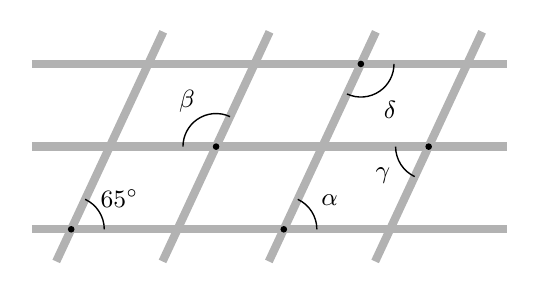
\begin{tikzpicture}[line width=0.7pt,font=\small]\draw[line width=3pt,black!30] (-0.5,0) -- (5.529,0);\draw[line width=3pt,black!30] (-0.5,1.05) -- (5.529,1.05);\draw[line width=3pt,black!30] (-0.5,2.1) -- (5.529,2.1);\draw[line width=3pt,black!30] (-0.19,-0.408) -- (1.169,2.508);\draw[line width=3pt,black!30] (1.16,-0.408) -- (2.519,2.508);\draw[line width=3pt,black!30] (2.51,-0.408) -- (3.869,2.508);\draw[line width=3pt,black!30] (3.86,-0.408) -- (5.219,2.508);\draw[black,line width=0.5pt] (0.42,0) arc (0:65:0.42);\node[inner sep=0pt] at (0.613,0.391) {$65^\circ$};\fill (0,0) circle (1.2pt);\draw[black,line width=0.5pt] (3.12,0) arc (0:65:0.42);\node[inner sep=0pt] at (3.282,0.371) {$\alpha$};\fill (2.7,0) circle (1.2pt);\draw[black,line width=0.5pt] (2.017,1.431) arc (65:180:0.42);\node[inner sep=0pt] at (1.469,1.632) {$\beta$};\fill (1.84,1.05) circle (1.2pt);\draw[black,line width=0.5pt] (4.12,1.05) arc (180:245:0.42);\node[inner sep=0pt] at (3.958,0.679) {$\gamma$};\fill (4.54,1.05) circle (1.2pt);\draw[black,line width=0.5pt] (3.502,1.719) arc (245:360:0.42);\node[inner sep=0pt] at (4.05,1.518) {$\delta$};\fill (3.679,2.1) circle (1.2pt);\end{tikzpicture}}{}{{\scriptsize\color{mbgrau}Ziel\hspace{2mm}}}
\medskip
\par\vspace{3mm}\setlength{\kr}{\dimexpr\pagegoal-\pagetotal-10mm\relax}%
\ifdim\kr>12mm\karomerk{k}{T}\noindent{\scriptsize\color{mbgrau}Platz zum Rechnen}\par\nointerlineskip\vspace{1mm}\noindent
\begin{tikzpicture}\clip (0,0) rectangle ({\linewidth-0.5mm},\kr);\draw[black!16,line width=0.3pt,step=5mm] (0,0) grid (\linewidth,\kr);\end{tikzpicture}\fi\par
\end{document}
